% This file was created with tikzplotlib v0.9.17.
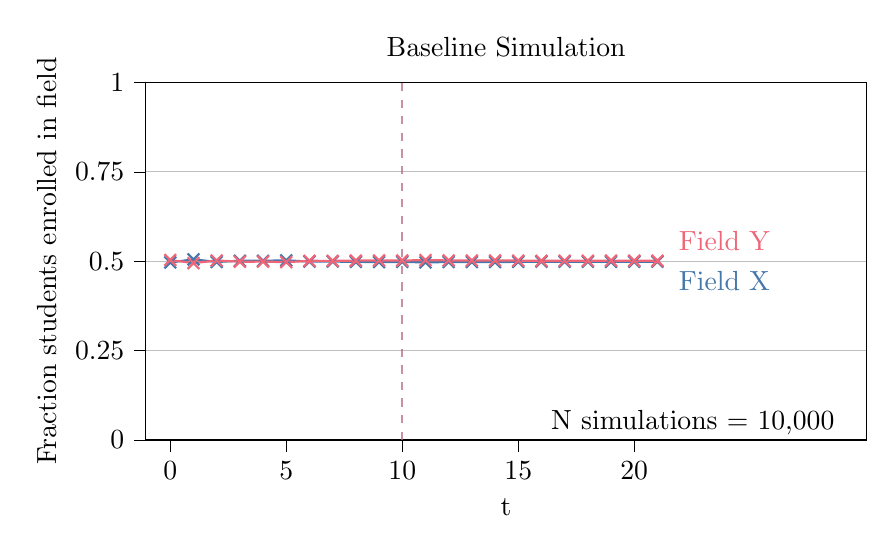
\begin{tikzpicture}

\definecolor{color0}{rgb}{0.266666666666667,0.466666666666667,0.666666666666667}
\definecolor{color1}{rgb}{0.933333333333333,0.4,0.466666666666667}

\begin{axis}[
height=6.121302808757603cm,
tick align=outside,
tick pos=left,
title={Baseline Simulation},
width=10.729849cm,
x grid style={white!69.0196078431373!black},
xlabel={t},
xmin=-1.05, xmax=30,
xtick style={color=black},
xtick={0,5,10,15,20},
xticklabels={
  \(\displaystyle 0\),
  \(\displaystyle 5\),
  \(\displaystyle 10\),
  \(\displaystyle 15\),
  \(\displaystyle 20\)
},
ylabel={Fraction students enrolled in field},
ymajorgrids,
ymin=0, ymax=1,
ytick style={color=black},
ytick={0,0.25,0.5,0.75,1},
yticklabels={
  \(\displaystyle 0\),
  \(\displaystyle 0.25\),
  \(\displaystyle 0.5\),
  \(\displaystyle 0.75\),
  \(\displaystyle 1\)
}
]
\addplot [thick, color0, mark=x, mark size=3, mark options={solid}]
table {%
0 0.4966
1 0.5052
2 0.498
3 0.5013
4 0.5011
5 0.5025
6 0.4989
7 0.4991
8 0.4983
9 0.4978
10 0.4981
11 0.4969
12 0.4978
13 0.498
14 0.4978
15 0.4983
16 0.4988
17 0.4987
18 0.4986
19 0.4983
20 0.4986
21 0.4987
};
\addplot [thick, color1, mark=x, mark size=3, mark options={solid}]
table {%
0 0.5034
1 0.4948
2 0.502
3 0.4987
4 0.4989
5 0.4975
6 0.5011
7 0.5009
8 0.5017
9 0.5022
10 0.5019
11 0.5031
12 0.5022
13 0.502
14 0.5022
15 0.5017
16 0.5012
17 0.5013
18 0.5014
19 0.5017
20 0.5014
21 0.5013
};
\addplot [semithick, color0, opacity=0.5, dashed]
table {%
10 0
10 1
};
\addplot [semithick, color1, opacity=0.5, dashed]
table {%
10 0
10 1
};
\draw (axis cs:21.5,0.4187) node[
  anchor=base west,
  text=color0,
  rotate=0.0
]{Field X};
\draw (axis cs:21.5,0.5313) node[
  anchor=base west,
  text=color1,
  rotate=0.0
]{Field Y};
\draw (axis cs:16,0.03) node[
  anchor=base west,
  text=black,
  rotate=0.0
]{N simulations = 10,000};
\end{axis}

\end{tikzpicture}
